\documentclass[11pt,a4paper]{article}

\usepackage[margin=1in]{geometry}
\usepackage{graphicx}
\usepackage{booktabs}
\usepackage{siunitx}
\usepackage{hyperref}
\usepackage{xcolor}
\usepackage{caption}
\usepackage{subcaption}
\usepackage{float}
\usepackage{microtype}
\usepackage{enumitem}

\graphicspath{{./}}
\sisetup{round-mode=places, round-precision=2}

\title{YOLOv8n Super-Resolution Evaluation on COCO val2017}
\author{HLCV Team~019 \\ Super Resolution Benchmark}
\date{15 July 2026}

\begin{document}
\maketitle

\begin{abstract}
We evaluate YOLOv8n object detection on the full COCO~val2017 set
(\num{5000} images) after controlled $2\times$ degradation
(Gaussian blur + bicubic downsampling), comparing four strategies:
raw low-resolution (baseline), ESPCN~$2\times$, FSRCNN~$2\times$, and
AnyUp (feature-level upsampling in the YOLO neck).
FSRCNN achieves the best mAP@0.5 (\SI{36.86}{\percent},
+\SI{1.72}{pp} vs.\ baseline). AnyUp underperforms baseline.
\end{abstract}

\tableofcontents
\vspace{1em}

%------------------------------------------------------------------------------
\section{Experimental setup}
\label{sec:setup}

\begin{table}[H]
\centering
\caption{Evaluation configuration (full validation set).}
\label{tab:setup}
\begin{tabular}{@{}ll@{}}
\toprule
\textbf{Item} & \textbf{Value} \\
\midrule
Detector & YOLOv8n (\texttt{yolov8n.pt}) \\
Dataset & COCO val2017, \textbf{5000 / 5000} images \\
LR input & \texttt{data/preprocessed/val2017\_lr\_x2} \\
Degradation & blur ($k{=}5$, $\sigma{=}2$) $\rightarrow$ bicubic $/2$ \\
Strategies & baseline, ESPCN\,$2\times$, FSRCNN\,$2\times$, AnyUp \\
Conf.\ threshold & $0.001$ (COCO-style PR) \\
Metric & mAP@0.5 (COCO bbox), by object size \\
Device & CPU (PyTorch CPU build) \\
\bottomrule
\end{tabular}
\end{table}

\paragraph{Pipeline.}
(1)~Offline HR$\rightarrow$LR downsample;
(2)~per-strategy image prep (identity / ESPCN / FSRCNN / AnyUp neck patch);
(3)~YOLO predict $\rightarrow$ COCO detections;
(4)~pycocotools mAP vs.\ original HR ground truth.

%------------------------------------------------------------------------------
\section{Full-val detection results}
\label{sec:results}

\begin{figure}[H]
\centering
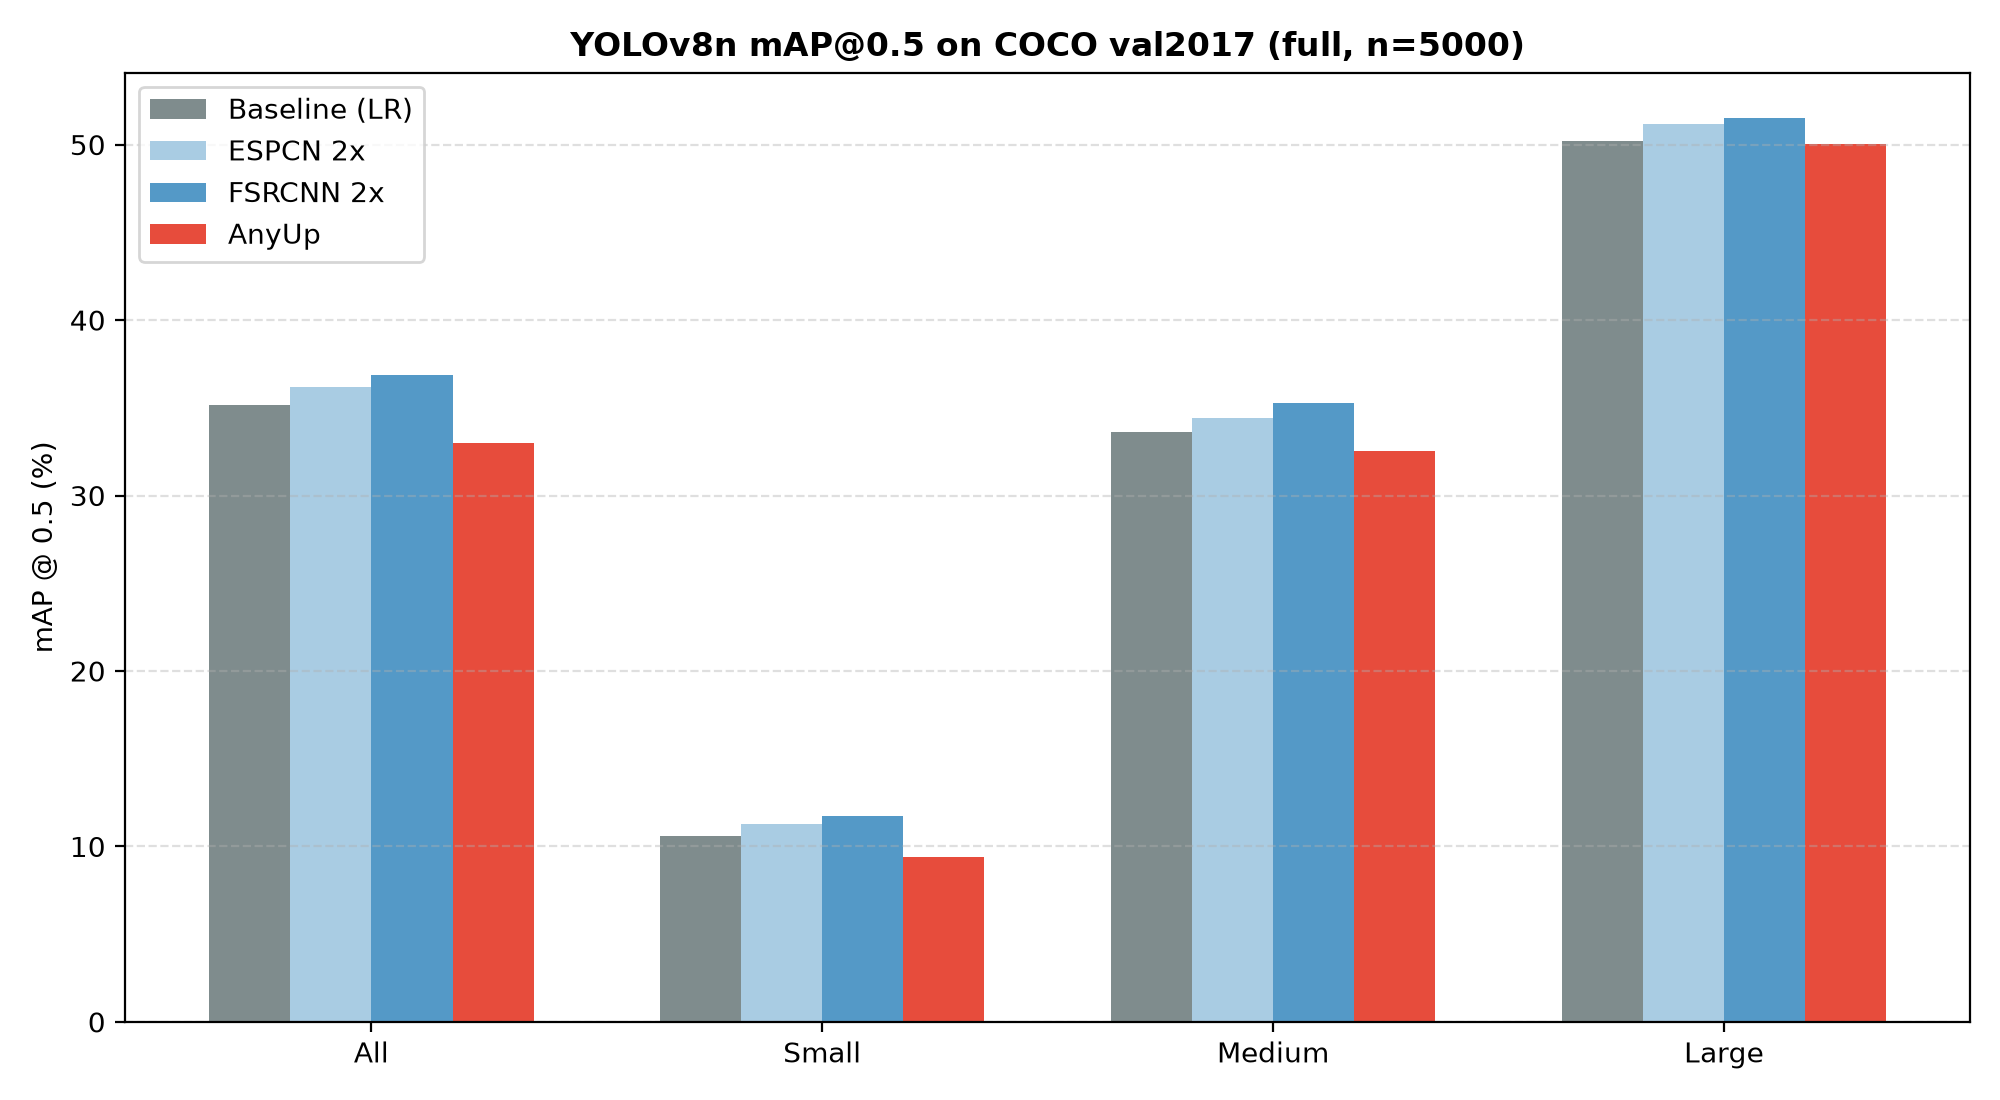
\includegraphics[width=\textwidth]{detection_map_corrected.png}
\caption{YOLOv8n mAP@0.5 on full COCO val2017
(\num{5000} images) for all SR strategies and object-size buckets.}
\label{fig:map}
\end{figure}

\subsection{Official results table}
\label{sec:official}

\begin{table}[H]
\centering
\caption{YOLOv8n mAP@0.5 on \textbf{full COCO val2017}
(\num{5000} images).}
\label{tab:map}
\begin{tabular}{@{}lrrrrrrr@{}}
\toprule
\textbf{Strategy}
  & \textbf{Images}
  & \textbf{Dets}
  & \textbf{All}
  & \textbf{Small}
  & \textbf{Medium}
  & \textbf{Large}
  & $\Delta$ All \\
\midrule
Baseline (LR) & 5000 & 658\,804 & 35.15 & 10.57 & 33.65 & 50.21 & --- \\
ESPCN $2\times$ & 5000 & 655\,883 & 36.21 & 11.27 & 34.41 & 51.15 & $+1.06$ \\
\textbf{FSRCNN $2\times$} & \textbf{5000} & \textbf{654\,593}
  & \textbf{36.86} & \textbf{11.73} & \textbf{35.30} & \textbf{51.52}
  & $\mathbf{+1.72}$ \\
AnyUp & 5000 & 519\,919 & 33.01 & 9.38 & 32.56 & 50.04 & $-2.14$ \\
\bottomrule
\end{tabular}
\end{table}

\begin{table}[H]
\centering
\caption{Exact mAP@0.5 values (fractional).}
\label{tab:map_exact}
\small
\begin{tabular}{@{}lcccc@{}}
\toprule
\textbf{Strategy} & mAP$_{50}$ All & Small & Medium & Large \\
\midrule
baseline & 0.351462 & 0.105669 & 0.336474 & 0.502096 \\
espcn2x  & 0.362126 & 0.112684 & 0.344090 & 0.511511 \\
fsrcnn2x & 0.368638 & 0.117259 & 0.352955 & 0.515243 \\
anyup    & 0.330139 & 0.093836 & 0.325611 & 0.500351 \\
\bottomrule
\end{tabular}
\end{table}

\paragraph{Takeaway.}
Pixel SR (ESPCN / FSRCNN) improves YOLOv8n on degraded COCO; FSRCNN is best.
AnyUp is below baseline, especially for small objects.

\subsection{Detection volume}

\begin{figure}[H]
\centering
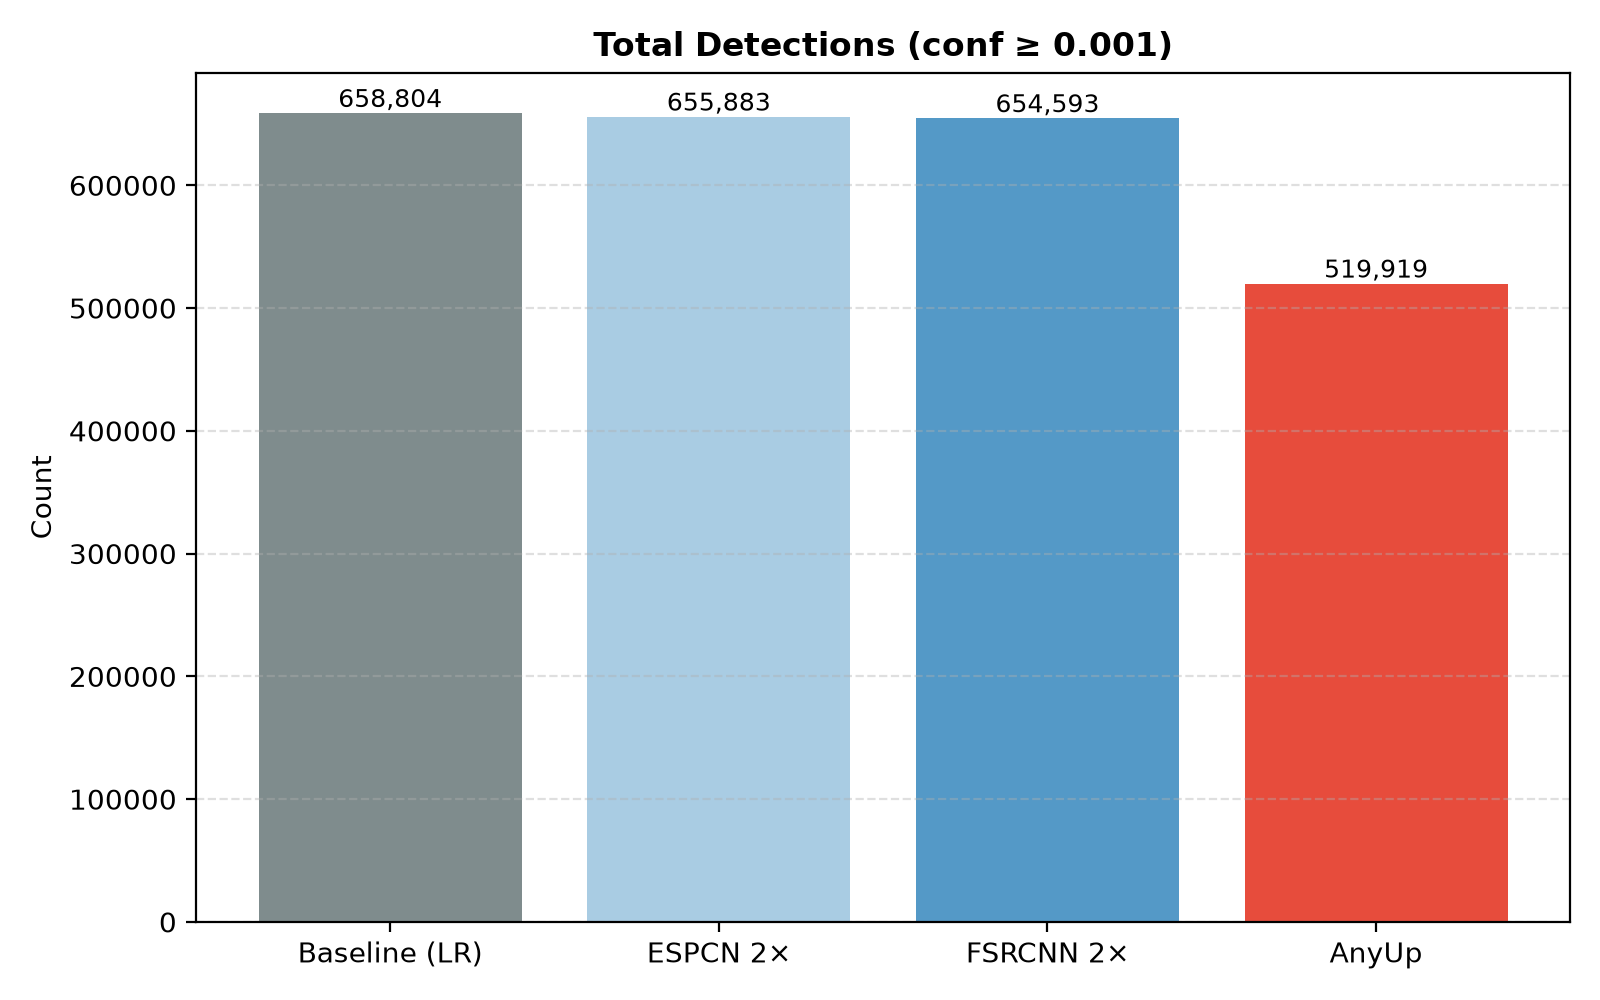
\includegraphics[width=0.85\textwidth]{detection_counts.png}
\caption{Total detections (conf.\ $\ge 0.001$) per strategy on full val2017.
AnyUp yields $\approx\SI{21}{\percent}$ fewer boxes than baseline.}
\label{fig:counts}
\end{figure}

%------------------------------------------------------------------------------
\section{Image degradation quality}
\label{sec:downsample}

Full val2017 downsample quality: HR vs.\ LR bicubic-upsampled back to HR
($n=\num{5000}$).

\begin{figure}[H]
\centering
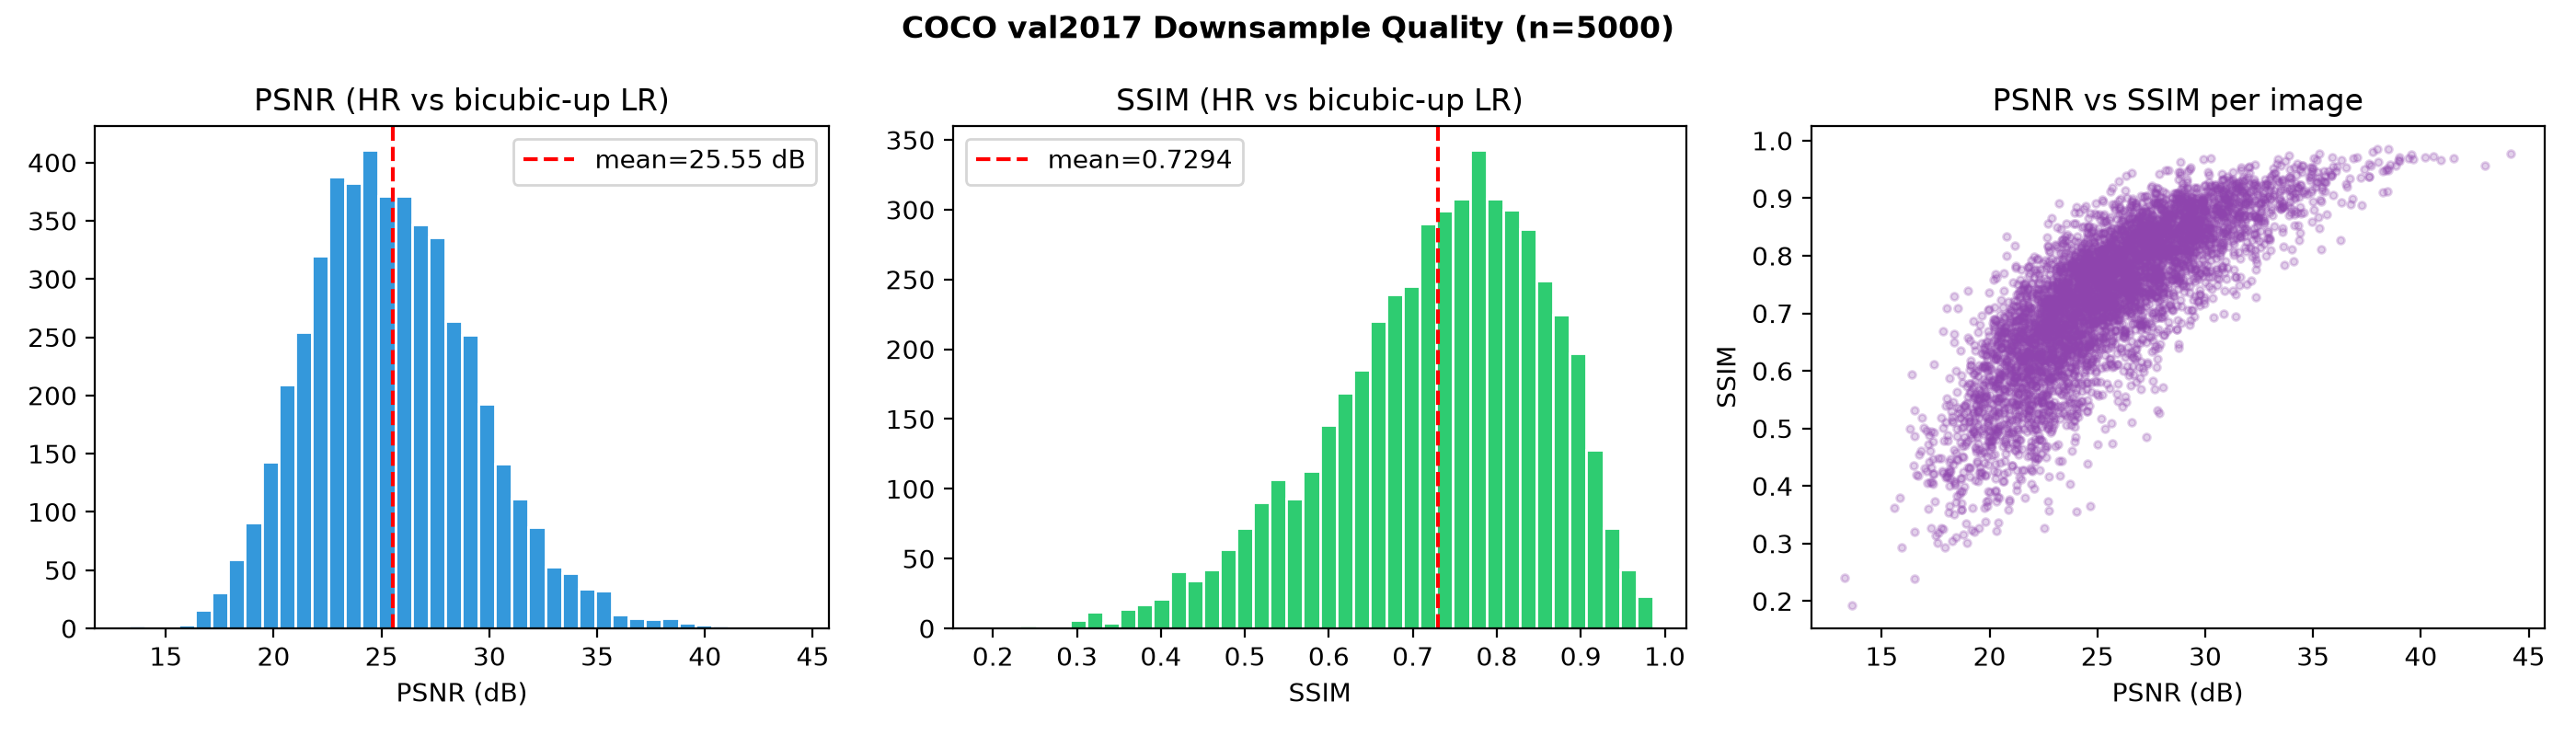
\includegraphics[width=\textwidth]{downsample_quality.png}
\caption{Downsample degradation on full COCO val2017:
PSNR / SSIM histograms and PSNR--SSIM scatter.
Mean PSNR $=\SI{25.55}{\decibel}$, mean SSIM $=0.7294$.}
\label{fig:downsample}
\end{figure}

\begin{table}[H]
\centering
\caption{Mean downsample quality (full val2017).}
\label{tab:downsample}
\begin{tabular}{@{}lr@{}}
\toprule
Metric & Mean \\
\midrule
PSNR & \SI{25.55}{\decibel} \\
SSIM & 0.7294 \\
\bottomrule
\end{tabular}
\end{table}

%------------------------------------------------------------------------------
\section{SR image quality (sample set)}
\label{sec:sr_quality}

Pixel SR quality on a small sample set
(\texttt{results/sr\_quality\_sample.json})---not full COCO, but ranking
matches detection performance.

\begin{figure}[H]
\centering
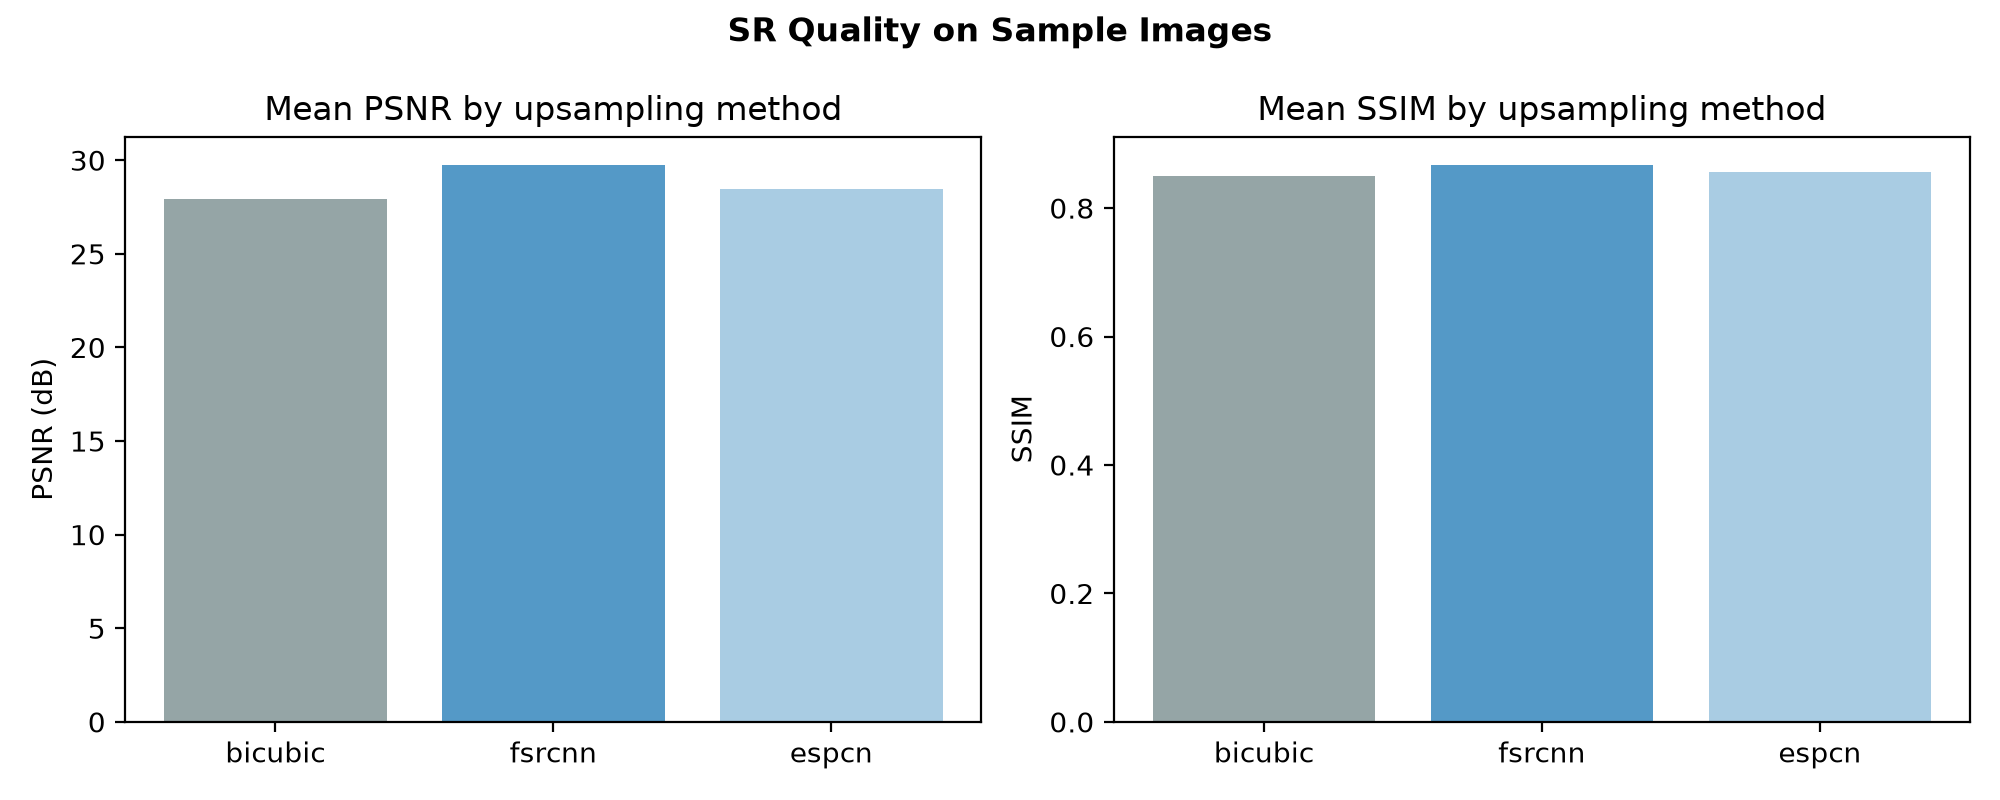
\includegraphics[width=0.9\textwidth]{sr_quality_sample.png}
\caption{Mean PSNR / SSIM for bicubic, FSRCNN, and ESPCN on sample images.
FSRCNN $>$ ESPCN $>$ bicubic.}
\label{fig:sr_quality}
\end{figure}

\begin{table}[H]
\centering
\caption{Sample-set SR quality.}
\label{tab:sr_quality}
\begin{tabular}{@{}lcc@{}}
\toprule
Method & Mean PSNR & Mean SSIM \\
\midrule
Bicubic & \SI{27.92}{\decibel} & 0.850 \\
ESPCN   & \SI{28.45}{\decibel} & 0.857 \\
FSRCNN  & \textbf{\SI{29.77}{\decibel}} & \textbf{0.868} \\
\bottomrule
\end{tabular}
\end{table}

%------------------------------------------------------------------------------
\section{SR quality vs.\ detection}
\label{sec:sr_vs_det}

\begin{figure}[H]
\centering
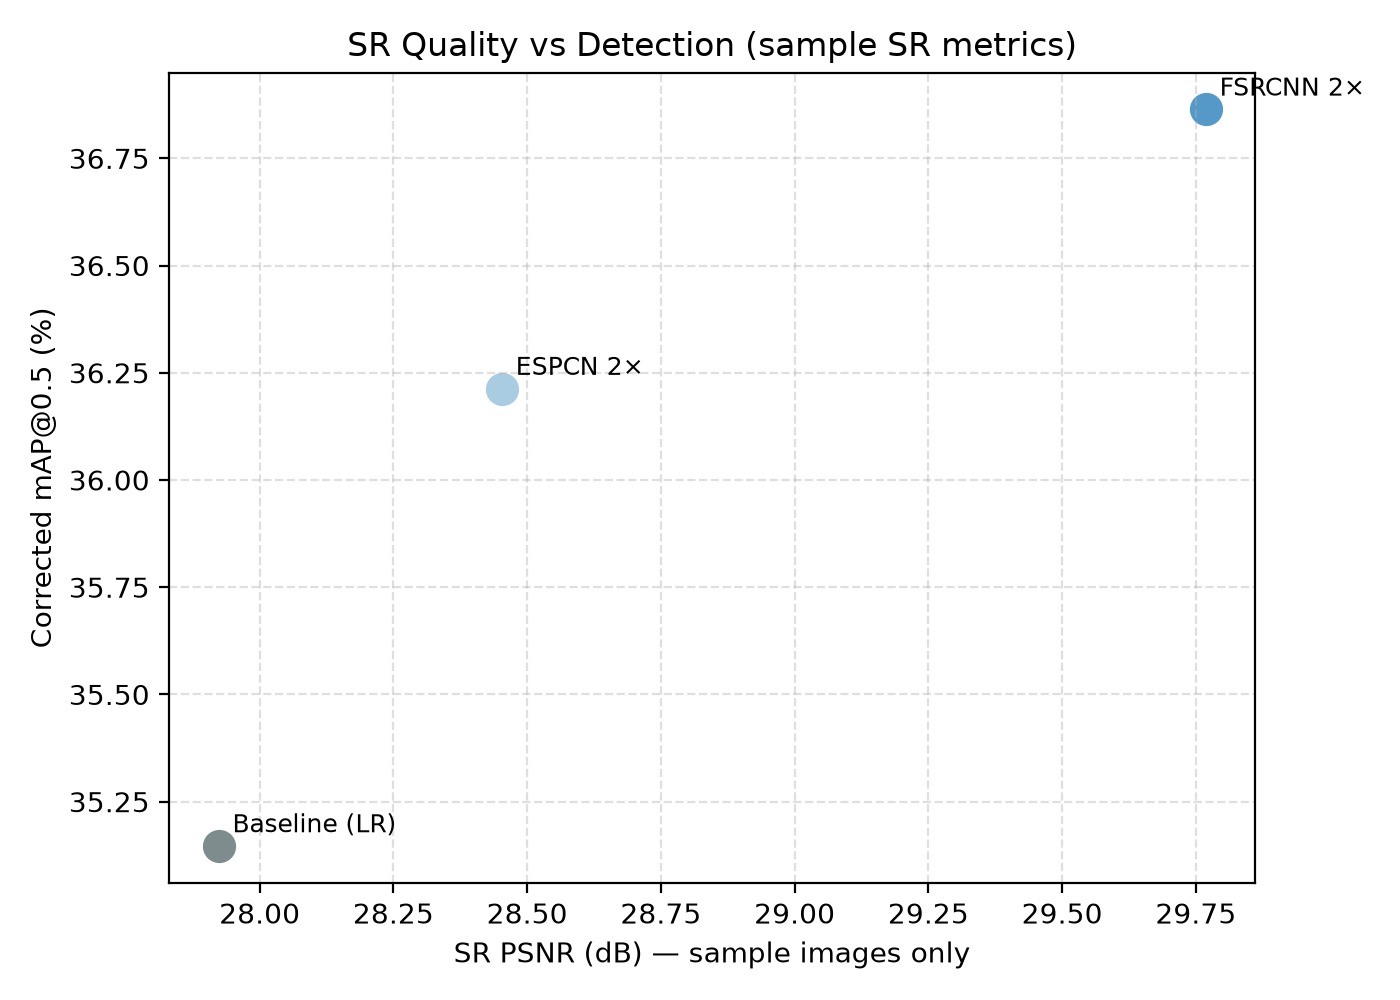
\includegraphics[width=0.75\textwidth]{sr_vs_detection.png}
\caption{Sample SR PSNR vs.\ full-val mAP@0.5.
Higher restoration quality tracks higher detection accuracy
(FSRCNN best). AnyUp omitted (feature-level SR, no pixel PSNR).}
\label{fig:sr_vs_det}
\end{figure}

\noindent
\textbf{Note:} sample PSNR and full-val detection use different image sets;
the trend is qualitative.

%------------------------------------------------------------------------------
\section{Strategy interpretation}
\label{sec:interp}

\begin{description}[style=nextline,leftmargin=*]
  \item[Baseline]
        Detect on degraded LR only. Control for ``no SR.''
  \item[ESPCN $2\times$]
        Modest PSNR/SSIM gains; $+\SI{1.06}{pp}$ mAP@0.5 overall;
        slightly better on small objects.
  \item[FSRCNN $2\times$]
        Best overall: $+\SI{1.72}{pp}$ all, $+\SI{1.16}{pp}$ small.
        Aligns with best sample SR quality.
  \item[AnyUp]
        Feature-level upsample in YOLO neck. Below baseline
        ($-\SI{2.14}{pp}$ all) and $\approx\SI{21}{\percent}$ fewer detections.
        Needs further tuning before claiming feature-SR benefits.
\end{description}

%------------------------------------------------------------------------------
\section{Reproducibility}
\label{sec:repro}

\paragraph{Artifacts.}
\begin{itemize}[leftmargin=*]
  \item Numbers: \texttt{analysis\_summary.json}
  \item Figures: \texttt{detection\_map\_corrected.png},
        \texttt{detection\_counts.png}, \texttt{downsample\_quality.png},
        \texttt{sr\_quality\_sample.png}, \texttt{sr\_vs\_detection.png}
  \item Regeneration: \texttt{python scripts/analyze\_results.py}
\end{itemize}

%------------------------------------------------------------------------------
\section{Conclusions}
\label{sec:concl}

\begin{enumerate}[leftmargin=*]
  \item On full COCO val2017 (\num{5000} images), FSRCNN is the strongest
        SR front-end for YOLOv8n (+1.72\,pp mAP@0.5 vs.\ baseline;
        Table~\ref{tab:map}).
  \item ESPCN also improves over baseline; AnyUp does not in the current setup.
  \item Optional next steps: HR upper-bound eval; YOLO fine-tune on
        FSRCNN inputs; Faster R-CNN / DETR under the same SR strategies.
\end{enumerate}

\end{document}
